\subsection {Session 8, Exercise 1}
\label{8_1}

\lineparagraph {Exercise}

Prove that $2-COLOR \prec 3-COLOR$ and that $3-COLOR \prec 100-COLOR$. What do these Karp-reductions say about the complexities of the three problems?

\lineparagraph {Solution}

The $n-COLOR$ problem, for any $n$ is the following:  For a given (undirected) $G$ graph, can the graph's vertices be correctly colored (=no edge-connected vertices get the same color) using $n$ colors? 

Let's do $2-COLOR \prec 3-COLOR$ first.

\separate
\separate

\textbf{First solution (existence of $NP \prec NP$-hard)}

This solution is pecific to the fact that the right side is NP-hard and the left side is NP, and that you only need to prove the existence of the Karp-reduction.

$2-COLOR$ is in $P$. To show that something is in $P$ we give a polynomial algorithm that can solve the problem.

The set of graphs that are $2$ colorable is called bipartite graphs, since these are the ones where the vertices can be grouped to set $A$ and set $B$ so that the edges are only running between sets.
x
To check if a graph is bipartite, we can run the BFS (Breadth-first search) algorithm. (You have learned this in Introduction to the Theory of Computing):

\begin{itemize}
    \item The algorithm returns a spanning tree (or forest, if the graph is not connected) of the graph, where the vertices are organized into layers of the tree (in the case of forest do the following for all trees = all connected parts of the graph separately).
    \item If we look at all of the edges from the graph (not just the edges that are part of the spanning tree), they can only run between consecutive layers, or inside the layers. 
    \item If there was an edge, that say went from layer $i$, to not layer $i$ or $i+1$, but $i+2$, $i+3$, etc, then the child in that edge should have been expanded on layer $i+1$, since BFS expands all unexplored connected vertices of a vertex on the next layer!
    \item A necessary and sufficient condition for a graph being bipartite is that it does not contain any odd cycles.
    \item How would an odd cycle look in this graph?
\end{itemize}

\begin{center}
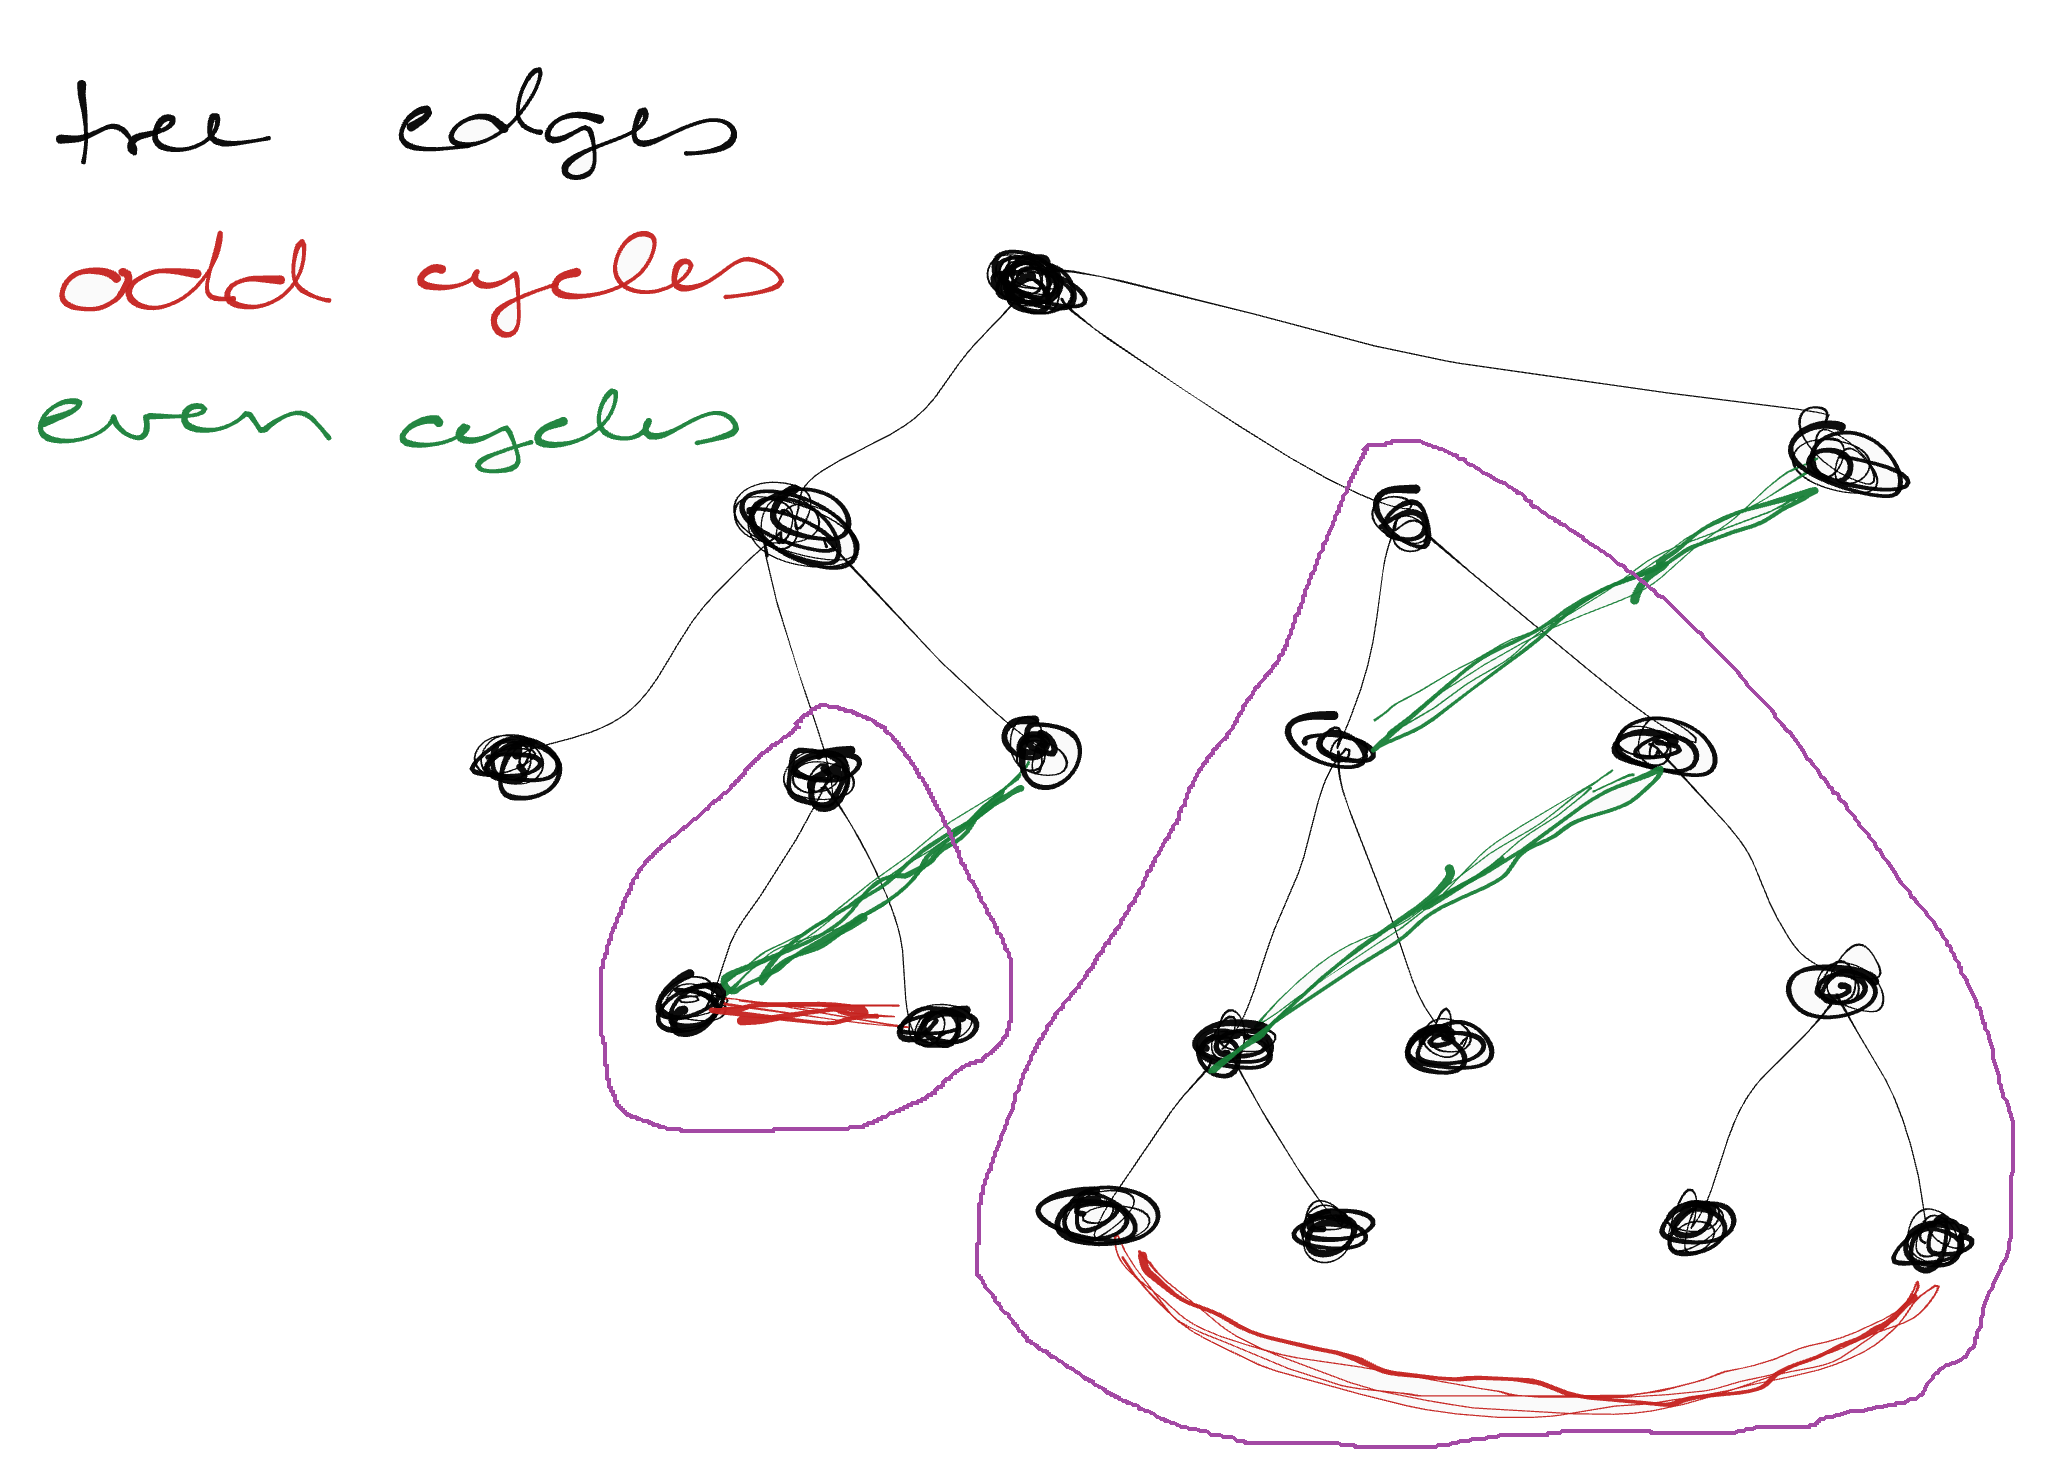
\includegraphics[width=0.8\linewidth]{./08/01/bipartite_bfs.png}
\end{center}

\begin{itemize}
    \item The edges of the tree are presented in black, while the other edges are either green (running between two layers), or red (running inside a layer).
    \item The problem edges are the red ones: if we look at their endpoints and trace them back up to their first common ancestor, we got ourselves an odd cycle. I have circled these with purple.
    \item The green edges will cause even cycles, which are bipartite (check this yourself!), so they are fine.
    \item So we have found that if the resulting tree has any red edge = any edge running inside a layer, then its not bipartite.
    \item BFS can be run in polynomial time and then we can check the endpoints of all of the edges, which layer they belong to in polynomial time as well.
\end{itemize}

So $2-COLOR$ is in $P$. However, starting from $3-COLOR$, up to any $n-COLOR$ where $3\leq{}n$, the problems are $NP$-complete. We have seen the $NP$-completeness of $3-COLOR$ on the lectures. When we need to prove that a Karp-reduction exists (as opposed to GIVE a Karp-reduction), it is not always necessary to actually give it. So the quickest way to prove that this Karp-reduction exists is the following:
\begin{itemize}
    \item $3-COLOR \in{} NP$-complete, which means it is both true that $3-COLOR \in{} NP$ , and $3-COLOR \in{} NP$-hard.
    \item Also $2-COLOR \in{} P \subseteq{} NP$.
    \item The definition of $NP$-hard is that a Karp-reduction exists from all languages that are in $NP$.
    \item So $2-COLOR \in{} NP$ and $3-COLOR \in{} NP$-hard means the $2-COLOR \prec 3-COLOR$ Karp reduction exists by definition.
\end{itemize}

\separate

\textbf{Second solution, specific to the fact that the left side is in $P$.}

We borrow the fact that $2-COLOR$ is in $P$, from the first solution, then we give a Karp-reduction using the fact that it is in $P$:

\begin{itemize}
    \item $2$-COLOR is in $P$, so there exists a polynomial time algorithm to solve it.
    \item Let's run this algorithm as the first step of our Karp-reduction! This is allowed, because we can run any polynomial transformation algorithm in a Karp-reduction.
    \item Now we know what the solution is, but the problem is that we can't directly return that. We must go through 3-COLOR, because the output from $3-COLOR$ is what we must use.
    \item Well, since we already know the solution, we can just make up two small graphs, one for which $3-COLOR$ answers $YES$ and another for which it answers $NO$. Then we can use those instead of our $YES$ / $NO$ answers to make $3-COLOR$ output exactly what we need. For example a single edge, for the $YES$ answer and a cycle of $3$ vertices for the $NO$ answer is good.
    \item Let's see this on the same Karp diagram:
\end{itemize}

\begin{center}
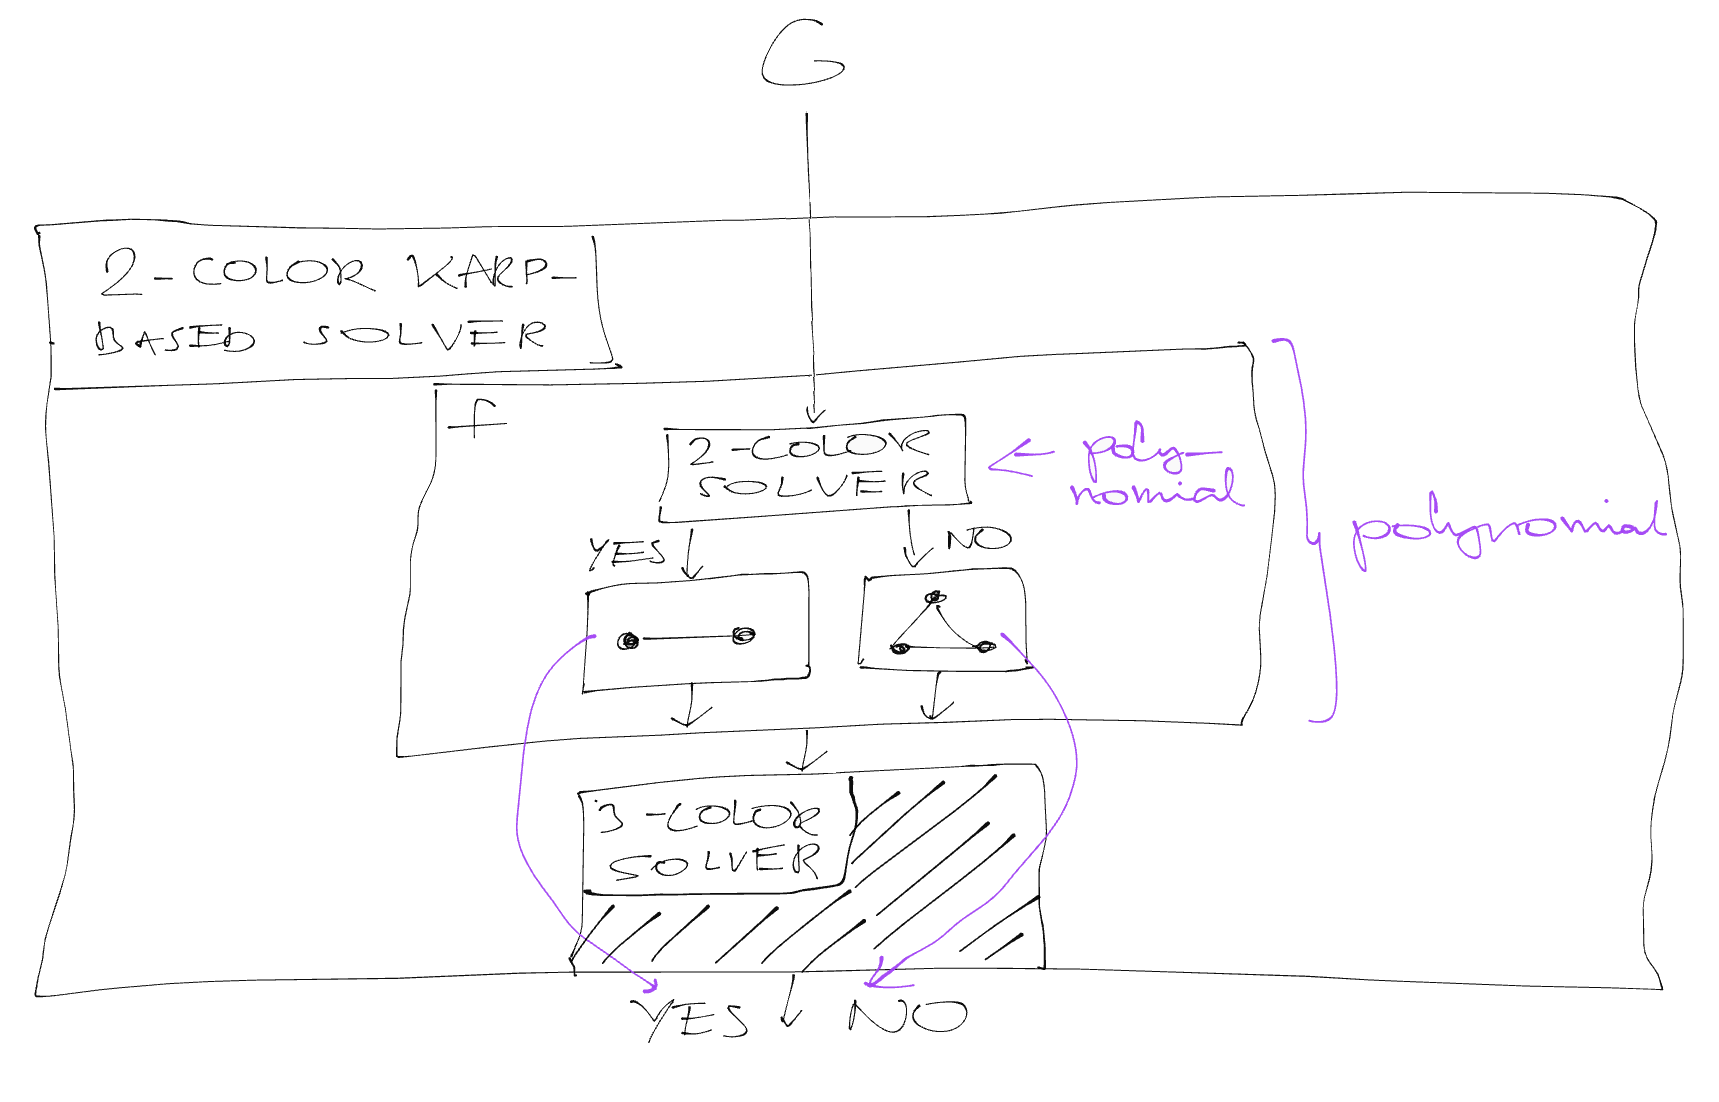
\includegraphics[width=0.8\linewidth]{./08/01/2color_3color_karp.png}
\end{center}

\separate

\textbf{Third solution, now specific to the coloring problem. :)}

\begin{itemize}
    \item Let's add one more vertex to the graph and connect that to every other vertex!
    \item This one vertex has to get a unique color, since it is connected to everything. We just wasted one of the colors from $3-COLOR$.
    \item Now $3-COLOR$ must give up one of its colors for the new vertex and try to color everything else using 2 colors which is just what we wanted.
    \item This transformation is polynomial, its adding a new row and column to the adjacency matrix and filling them with 1's, except for the bottom right corner, which is zero.
    \item If there is a 2-coloring in $G$, then there will be a 3-coloring in $G'$, since the one extra vertex can get the third color.
    \item If there is no 2-coloring in $G$, then there cant be any 3-coloring of $G'$, since if there were a correct 3-coloring in $G'$, then the new vertex must get a unique color, since it is connected to everything, so the other vertices can only get 2 other colors, so this would be a correct 2-coloring of $G$, which is a contradiction.
\end{itemize}

The solution to $3-COLOR \prec 100-COLOR$ is similar to the previous ones:

\begin{itemize}
    \item First solution: $3-COLOR$ and $100$-COLOR are both $NP$-complete, so they are both in $NP$ and in $NP$-hard. Use the $NP$ fact for $3-COLOR$ and the $NP$-hard fact for $100-COLOR$, then it's the same argument as in the previous part.
    \item Second solution: We can't do this, since $3-COLOR$ is not in $P$. :(
    \item Third solution: We need to waste 97 colors, this can be done by adding a fully connected graph of 97 vertices to $G$, which is traditionally denoted by $K_{97}$ and also connecting all of $K_{97}$'s vertices to all of $G$'s vertices. (So full bipartite graph between these two.) Then, the same argument works as previously.
\end{itemize}